%% FullCourse_10Lecs -- Lecture 9, Topic 9.5: Tracing + Mistakes/Limits/Security + Managing Context
%% Source: ./archive_pre_split/Lec09_Agentic_AI_v3.tex (sections 9-11)
%% FullCourse-only content: Context Dilemma section (not in MiniCourse).
%% Rewritten 2026-07-06: Act 5 "Mindset" of the five-act structure. Adds the fellows
%%         honest-negative-result failure case (Lec10 T4); compaction mechanics moved
%%         to T2, trade-off kept here; Context Dilemma compressed ~14 -> 6 frames;
%%         closes with the HA-Ramsey paradigm-shift frame (Lec10 T8 F37/F31) and the
%%         "Your Job Description" map reprise. See Lec09_Rewrite_Plan_2026-07-06.md.

%% Shared preamble for the FullCourse_10Lecs topic decks.
%%
%% Each topic .tex \input's this file, then defines its own \title, \date
%% override (if any), \graphicspath, and \begin{document}.
%%
%% Reconstructed verbatim from the inlined copy preserved in
%% Lec10_Case_Studies/Lec10_T8_Case6_DeepRamsey.tex (lines 23-190), which is
%% explicitly annotated there as "from ../shared_preamble.tex, copied verbatim".
%% Base preamble matches MiniCourse_8hr/Slides/shared_preamble.tex; this version
%% additionally provides \sectiondivider, the conceptbox/cautionbox/examplebox/
%% takeawaybox tcolorboxes, and \compacttables used across the split decks.

\documentclass[10pt,english,aspectratio=169]{beamer}

\usepackage{ae,aecompl}
\usepackage[T1]{fontenc}
\usepackage{textcomp}
\usepackage[utf8]{inputenc}
\usepackage{babel}
\usepackage{datetime2}

\setcounter{secnumdepth}{3}
\setcounter{tocdepth}{3}

\usepackage{amsmath, amssymb, amsthm, graphicx}
\usepackage{booktabs, multirow}
\usepackage{tikz}
\usepackage{pgfplots}
\pgfplotsset{compat=1.16}
\usepackage[most]{tcolorbox}
\tcbuselibrary{skins, breakable, theorems}
\usepackage{listings}
\usepackage{xcolor}

\lstset{
  basicstyle=\ttfamily\small,
  keywordstyle=\color{blue!80!black}\bfseries,
  commentstyle=\color{green!50!black}\itshape,
  stringstyle=\color{orange!80!black},
  backgroundcolor=\color{gray!8},
  frame=single,
  rulecolor=\color{gray!40},
  breaklines=true,
  showstringspaces=false,
  numbers=none,
}

\lstdefinestyle{pythonstyle}{
    language=Python,
    basicstyle=\ttfamily\footnotesize,
    keywordstyle=\color{blue!80!black}\bfseries,
    commentstyle=\color{green!50!black}\itshape,
    stringstyle=\color{orange!80!black},
    frame=single,
    breaklines=true,
    showstringspaces=false,
    numbers=left,
    numbersep=5pt,
    numberstyle=\tiny\color{gray},
    backgroundcolor=\color{gray!8},
    rulecolor=\color{gray!40}
}

\ifx\hypersetup\undefined
  \AtBeginDocument{%
    \hypersetup{bookmarks=false,breaklinks=true,pdfborder={0 0 0},colorlinks=true,
      linkcolor=DarkText,urlcolor=RedTitle}%
  }
\else
  \hypersetup{bookmarks=false,breaklinks=true,pdfborder={0 0 0},colorlinks=true,
    linkcolor=DarkText,urlcolor=RedTitle}%
\fi

\makeatletter
\newcommand\makebeamertitle{%
  \begin{frame}[plain]
    \vspace*{1.0cm}
    \centering
    {\usebeamerfont{title}\usebeamercolor[fg]{title}\inserttitle\par}
    \vspace{1.0cm}
    {\usebeamerfont{author}\usebeamercolor[fg]{author}\insertauthor\par}
    \vspace{0.2cm}
    {\usebeamerfont{date}\usebeamercolor[fg]{date}\insertdate\par}
  \end{frame}}%
\AtBeginDocument{%
  \let\origtableofcontents=\tableofcontents
  \def\tableofcontents{\@ifnextchar[{\origtableofcontents}{\gobbletableofcontents}}
  \def\gobbletableofcontents#1{\origtableofcontents}%
}

\usetheme{metropolis}
\usefonttheme{professionalfonts}

\definecolor{LightGray}{RGB}{230,230,230}
\definecolor{RedTitle}{RGB}{0,0,200}
\definecolor{VeryLightGray}{RGB}{245,245,245}
\definecolor{DarkText}{RGB}{0,0,0}

\setbeamercolor{background canvas}{bg=white}
\setbeamercolor{title}{fg=RedTitle}
\setbeamercolor{author}{fg=DarkText}
\setbeamercolor{date}{fg=DarkText}
\setbeamercolor{frametitle}{bg=VeryLightGray,fg=DarkText}
\setbeamercolor{normal text}{fg=DarkText}
\setbeamerfont{title}{size=\large}

\setbeamersize{text margin left=5mm, text margin right=5mm}
\addtobeamertemplate{frametitle}{}{\vspace{-0.5em}}
\newcommand{\reducevspace}{\vspace{-0.5cm}}

% Shared section divider and box styles for split topic decks.
\newcommand{\sectiondivider}[2]{%
\begin{frame}[plain,noframenumbering]
\begin{center}
\vfill
{\Large\textbf{#1}\par}
\vspace{0.35cm}
{\normalsize #2\par}
\vfill
\end{center}
\end{frame}
}

\newtcolorbox{conceptbox}[1][]{
  colback=blue!3,
  colframe=RedTitle!55,
  boxrule=0.35mm,
  arc=1mm,
  left=2mm,
  right=2mm,
  top=1mm,
  bottom=1mm,
  #1
}
\newtcolorbox{cautionbox}[1][]{
  colback=red!3,
  colframe=red!50!black,
  boxrule=0.35mm,
  arc=1mm,
  left=2mm,
  right=2mm,
  top=1mm,
  bottom=1mm,
  #1
}
\newtcolorbox{examplebox}[1][]{
  colback=green!3,
  colframe=green!45!black,
  boxrule=0.35mm,
  arc=1mm,
  left=2mm,
  right=2mm,
  top=1mm,
  bottom=1mm,
  #1
}
\newtcolorbox{takeawaybox}[1][]{
  colback=VeryLightGray,
  colframe=RedTitle!55,
  boxrule=0.35mm,
  arc=1mm,
  left=2mm,
  right=2mm,
  top=1mm,
  bottom=1mm,
  #1
}
\newcommand{\compacttables}{\renewcommand{\arraystretch}{1.15}}

\setbeamertemplate{navigation symbols}{}
\setbeamertemplate{footline}{%
  \hfill%
  \usebeamercolor[fg]{page number in head/foot}%
  \usebeamerfont{page number in head/foot}%
  \insertframenumber\,/\,\inserttotalframenumber\kern1em\vskip2pt%
}

\makeatother

\author{Zhigang Feng}
% "date with time": compile timestamp so each build is identifiable.
\date{\today\ \DTMcurrenttime}


% Suppress redundant auto-generated metropolis section page; \sectiondivider frames are the dividers we keep.
\metroset{sectionpage=none}

\graphicspath{{./pic/}{./figures/}{../../MiniCourse_8hr/Slides/Module4_Agentic_AI/pic/}{../}}


\usetikzlibrary{positioning,arrows.meta,shapes,calc}

%% Lec09 shared MAP slide: "one map, five acts" recurring diagram.
%% Input this file AFTER ../shared_preamble.tex (needs RedTitle, VeryLightGray)
%% and call \LecNineMap{k} inside a frame, where k in {1..5} highlights the
%% current act ("you are here") and k = 0 renders the closing reprise with all
%% five acts checked (used by T5's "Your Job Description" frame).
%% Filename deliberately does not match the build glob Lec*_T*.tex, so the
%% build script never tries to compile it standalone.

\newcommand{\LecNineMap}[1]{%
% Precompute per-box style selectors and the checkmark token; TikZ option
% lists are comma-split before TeX conditionals run, so \ifnum must not sit
% inside a [...] options list.
\ifnum#1=0
  \tikzset{lecmapa/.style={lecmapdone}, lecmapb/.style={lecmapdone},
           lecmapc/.style={lecmapdone}, lecmapd/.style={lecmapdone},
           lecmape/.style={lecmapdone}}%
  % green fill + the "all five acts complete" banner mark completion; a per-box
  % checkmark overflows the MANAGEMENT box, so keep the token empty here too.
  \def\lecmapchk{}%
\else
  \tikzset{lecmapa/.style={}, lecmapb/.style={}, lecmapc/.style={},
           lecmapd/.style={}, lecmape/.style={}}%
  \def\lecmapchk{}%
  \ifnum#1=1 \tikzset{lecmapa/.style={lecmapcur}}\fi
  \ifnum#1=2 \tikzset{lecmapb/.style={lecmapcur}}\fi
  \ifnum#1=3 \tikzset{lecmapc/.style={lecmapcur}}\fi
  \ifnum#1=4 \tikzset{lecmapd/.style={lecmapcur}}\fi
  \ifnum#1=5 \tikzset{lecmape/.style={lecmapcur}}\fi
\fi
\begin{center}
\begin{tikzpicture}[
    act/.style={rectangle, rounded corners, draw=black!60, fill=VeryLightGray,
        minimum width=2.6cm, minimum height=0.92cm, text width=2.5cm,
        align=center, font=\scriptsize, text=DarkText},
    lecmapcur/.style={draw=RedTitle, very thick, fill=orange!20},
    lecmapdone/.style={draw=green!45!black, thick, fill=green!10},
    q/.style={font=\tiny\itshape, text width=2.7cm, align=center, text=black!70},
    sat/.style={rectangle, rounded corners, draw=black!45, dashed, fill=white,
        text width=5.0cm, align=center, font=\tiny, text=black!70,
        minimum height=0.5cm},
    barlab/.style={font=\tiny\bfseries, text=black!60},
    arr/.style={-{Stealth[length=2mm]}, thick, gray!60}
]
    % --- five act boxes ---
    \node[act, lecmapa] (a1) at (0,0)
        {\textbf{9.1 MAP}\lecmapchk\\ \tiny what \& why};
    \node[act, lecmapb] (a2) at (2.85,0)
        {\textbf{9.2 MACHINE}\lecmapchk\\ \tiny under the hood};
    \node[act, lecmapc] (a3) at (5.7,0)
        {\textbf{9.3 METHOD}\lecmapchk\\ \tiny homotopy workflow};
    \node[act, lecmapd] (a4) at (8.55,0)
        {\textbf{9.4 MANAGEMENT}\lecmapchk\\ \tiny run the project};
    \node[act, lecmape] (a5) at (11.4,0)
        {\textbf{9.5 MINDSET}\lecmapchk\\ \tiny your role};
    \draw[arr] (a1) -- (a2);
    \draw[arr] (a2) -- (a3);
    \draw[arr] (a3) -- (a4);
    \draw[arr] (a4) -- (a5);
    % --- the student question each act answers ---
    \node[q] at (0,-0.82)    {what is this,\\ and why care?};
    \node[q] at (2.85,-0.82) {how does it work?\\ how do I start?};
    \node[q] at (5.7,-0.82)  {how do I structure\\ real work?};
    \node[q] at (8.55,-0.82) {how do I run a\\ whole project?};
    \node[q] at (11.4,-0.82) {what goes wrong?\\ what is my job?};
    % --- "you are here" marker above the current act ---
    \ifnum#1=1 \node[font=\scriptsize\bfseries, text=RedTitle] at (0,0.95)
        {you are here\ $\blacktriangledown$};\fi
    \ifnum#1=2 \node[font=\scriptsize\bfseries, text=RedTitle] at (2.85,0.95)
        {you are here\ $\blacktriangledown$};\fi
    \ifnum#1=3 \node[font=\scriptsize\bfseries, text=RedTitle] at (5.7,0.95)
        {you are here\ $\blacktriangledown$};\fi
    \ifnum#1=4 \node[font=\scriptsize\bfseries, text=RedTitle] at (8.55,0.95)
        {you are here\ $\blacktriangledown$};\fi
    \ifnum#1=5 \node[font=\scriptsize\bfseries, text=RedTitle] at (11.4,0.95)
        {you are here\ $\blacktriangledown$};\fi
    \ifnum#1=0 \node[font=\scriptsize\bfseries, text=green!45!black] at (5.7,0.95)
        {all five acts complete};\fi
    % --- bottom band: the three questions of the lecture ---
    \fill[blue!10]   (-1.3,-1.55) rectangle (4.15,-1.22);
    \fill[green!10]  (4.4,-1.55)  rectangle (9.85,-1.22);
    \fill[orange!15] (10.1,-1.55)  rectangle (12.7,-1.22);
    \node[barlab] at (1.425,-1.385)  {HOW IT WORKS};
    \node[barlab] at (7.125,-1.385)  {HOW TO USE IT WELL};
    \node[barlab] at (11.4,-1.385)   {YOUR ROLE};
    % --- dashed satellites: the two decks outside these five acts ---
    \node[sat] at (2.0,-2.2)
        {\textit{after 9.1:} optional interlude \textbf{9.1b} --- the agent landscape (MCP, A2A, benchmarks, safety)};
    \node[sat] at (9.8,-2.2)
        {\textit{after 9.5:} \textbf{9.6} wrap-up $\to$ \textbf{Lec10} full case studies (same morning)};
\end{tikzpicture}
\end{center}
}


\title[AI for Econ Research]{AI for Economic Research: Dynamic Models, Language, and Agents\\
Lecture 9.5: Tracing, Mistakes, and Managing Context --- Your Role as Researcher}

\begin{document}

\makebeamertitle

%=============================================================================
\begin{frame}{The Map: Act 5 --- The Mindset}
\textbf{This deck answers the last question: what can go wrong, and what exactly is my job?}

\LecNineMap{5}

\vspace{0.1cm}
\footnotesize\textit{Route: audit what the agent actually did (tracing) $\to$ the failure modes the harness cannot prevent $\to$ managing context: the compaction trade-off and the Context Dilemma $\to$ the paradigm shift, completed --- what AI changed and what stays yours.}
\end{frame}

%=============================================================================
\section{Tracing}
%===========================================================

\sectiondivider{Tracing}{Audit what the agent actually did}

\begin{frame}{The Anchor Returns: Aiyagari Through the Full Harness}
\textbf{Household problem}
\[
c_t + a_{t+1} = (1+r)a_t + wz_t, \qquad a_{t+1} \geq \underline{a}
\]
with idiosyncratic productivity $z_t$ following a Markov chain.

\vspace{0.2cm}

\textbf{Why it is a good lecture example}
\begin{itemize}
    \item it is the cleanest computational example in the course
    \item it admits a clean V0 $\to$ V1 $\to$ V2 progression
    \item it has obvious validation checkpoints that generalize to other workflows
\end{itemize}

\vspace{0.2cm}

\textbf{Where we are:} this project climbed T3's ladder inside T4's project objects. Now we audit the run --- because delegation without auditing is abdication.
\end{frame}

\begin{frame}[fragile]{Tracing (1): The File Flow}
\begin{lstlisting}[style=pythonstyle,language={},basicstyle=\ttfamily\scriptsize]
1. Read CLAUDE.md
2. Read any relevant rules
3. Load /solve-model from SKILL.md
4. Read references/aiyagari-guide.md
5. Write plan or update quality_reports/
6. Edit scripts/aiyagari_v0.py
7. Run verifier and reviewers
8. Save outputs and logs
\end{lstlisting}

\vspace{0.2cm}

\textbf{What students should notice:} the workflow is file-driven. The agent is acting inside a structured research project, not improvising in a vacuum --- and every step above leaves an inspectable trace.
\end{frame}

\begin{frame}[fragile]{Tracing (2): The Orchestrator Loop}
\begin{lstlisting}[style=pythonstyle,language={},basicstyle=\ttfamily\scriptsize]
You type: /solve-model aiyagari v1

Plan:
  read project instructions
  restate the target
  implement bounded changes

Review loop:
  run verifier
  run code reviewer
  run domain reviewer
  fix issues that matter
  report what changed and what passed
\end{lstlisting}

\vspace{0.2cm}

\textbf{This is the core advantage of the harness:} the review sequence is not a remembered prompt. It is part of the saved workflow.
\end{frame}

\begin{frame}[fragile]{Tracing (3): Inside \texttt{CLAUDE.md}}
\begin{lstlisting}[style=pythonstyle,language={},basicstyle=\ttfamily\tiny,numbers=none]
# CLAUDE.md
Project: Aiyagari workflow for lecture 9
Goal: build v0, v1, and v2 sequentially
Outputs: policies, stationary distribution, diagnostics
Conventions: save figures to output/ and plans to quality_reports/
Validation: do not move to the next version until benchmarks pass
\end{lstlisting}

\vspace{0.2cm}

\textbf{If the file is good,} the project can survive a fresh session, a new RA, or a change in agent tool.
\end{frame}

\begin{frame}[fragile]{Tracing (4): Inside \texttt{SKILL.md} and the Reference Guide}
\begin{columns}[T]
\begin{column}{0.48\textwidth}
\textbf{\texttt{SKILL.md}}
\begin{lstlisting}[style=pythonstyle,language={},basicstyle=\ttfamily\tiny,numbers=none]
name: solve-model
description: build and validate

Steps:
1. Read the model guide
2. Write or update a plan
3. Implement one version
4. Run required checks
5. Save outputs and report
\end{lstlisting}
\end{column}
\begin{column}{0.48\textwidth}
\textbf{\texttt{aiyagari-guide.md}}
\begin{lstlisting}[style=pythonstyle,language={},basicstyle=\ttfamily\tiny,numbers=none]
V0: deterministic benchmark
V1: add Markov income risk
V2: compute stationary dist.

Checks:
- zero-variance limit
- sensible mass at a_min
- stable diagnostics
\end{lstlisting}
\end{column}
\end{columns}

\vspace{0.2cm}

\textbf{Interpretation:} the skill stores the protocol; the reference guide stores the model detail.

\vspace{0.05cm}
\footnotesize\textit{Capstone note: this pair is the skeleton of a Track D2 deliverable --- a validated skill for a recurring research task.}
\end{frame}

%===========================================================
%=============================================================================
\section{Mistakes, Limits, and Security}
%===========================================================

\sectiondivider{Mistakes, Limits, and Security}{What can go wrong and how to stay disciplined}

\begin{frame}{Three Recurring Operator Mistakes}
\textbf{The most common ways an agent project goes off the rails.}

\vspace{0.2cm}

\begin{itemize}
    \item \textbf{Mistake 1: Treating Git as optional.} Agents are most useful when experimentation is reversible. Git provides the audit trail and the emergency brake. If you would be unhappy losing the current project state, put it under Git before using an agent aggressively.
    \medskip
    \item \textbf{Mistake 2: Underusing skills.} Economists repeat many workflows (clean data, validate tables, prepare slides, review code). Repeated work should move from chat into a saved protocol --- otherwise the same task is re-explained every week and interpreted slightly differently each time.
    \medskip
    \item \textbf{Mistake 3: One giant thread.} Long conversations accumulate stale context: planning, debugging, and revision all mix together, and the model pays attention to constraints that no longer matter. Plan the task, save the plan, then start a cleaner execution session. \textit{(The Managing Context section shows exactly why this fails.)}
\end{itemize}
\end{frame}

\begin{frame}{Where Terminal Agents Still Fail}
\begin{itemize}
    \item Long-context drift: an early constraint gets forgotten
    \item Econometric edge cases: wrong clustering level, wrong sample restriction, weak-instrument issues
    \item Hallucinated APIs or package arguments
    \item Happy-path scripts that fail on messy data
    \item Oscillating fix loops on stubborn bugs
\end{itemize}

\vspace{0.3cm}

\textbf{The output may look polished even when the economics is wrong.} That is why validation stays central. The next three frames show concrete instances.
\end{frame}

\begin{frame}[fragile]{Failure Case 1: Clustering Standard Errors}
\textbf{Prompt:} ``Estimate the effect of minimum-wage increases on teen employment using county--month panel data.''

\vspace{0.12cm}
\begin{lstlisting}[basicstyle=\ttfamily\scriptsize,numbers=none]
* Agent default:
reg emp_teen mw_increase i.county i.month, robust
\end{lstlisting}

\vspace{0.08cm}
\begin{itemize}
    \item \textbf{What's wrong.} Identification is at the county level, so standard errors must cluster at county. The default \texttt{,~robust} is technically valid syntax but econometrically wrong here; SEs will be 2--4$\times$ too small.
    \item \textbf{Why the agent missed it.} The training corpus rewards code that \emph{runs}; clustering choice is a research-design decision, not a code-syntax decision.
    \item \textbf{Detection.} Always specify the clustering level in the prompt; cross-check against the canonical reference (Abadie, Athey, Imbens, Wooldridge 2023, \emph{QJE}, ``When Should You Adjust Standard Errors for Clustering?'').
    \item \textbf{Hook it.} A repository rule that requires every regression to declare a clustering level catches this category at the source.
\end{itemize}
\end{frame}

\begin{frame}[fragile]{Failure Case 2: The CPI-1983 Definitional Break}
\textbf{Prompt:} ``Merge FRED series UNRATE and CPIAUCSL, both monthly, 1948 to present.''

\vspace{0.12cm}
\begin{lstlisting}[basicstyle=\ttfamily\scriptsize,numbers=none]
* Agent default:
pd.merge(unrate, cpi, on="date", how="inner")
\end{lstlisting}

\vspace{0.08cm}
\begin{itemize}
    \item \textbf{What's wrong.} CPIAUCSL carries a \emph{methodological} break: effective Jan 1983, BLS switched owner-occupied housing in CPI-U to \emph{rental equivalence} (owners' equivalent rent). Level and base (1982--84$=$100) are continuous, so nothing looks broken --- but pre- and post-1983 measure shelter differently; a regression on the merged span treats two definitions as one variable.
    \item \textbf{Why the agent missed it.} Happy-path code works on the dominant case; definitional breaks leave units and base unchanged, so nothing fails visibly.
    \item \textbf{Detection.} Audit the data (\texttt{describe()}, plots, rows by year) and read the series' definition notes \emph{before} regressing; encode the break-audit as a rule.
\end{itemize}
\end{frame}

\begin{frame}{Failure Case 3: When the Data Says No --- 882 Fellows}
\textbf{The fellows thread ends with the most instructive failure of all: one that no amount of agent power could fix.}

\vspace{0.15cm}

\begin{examplebox}
\small
The instructor's full scan parsed \textbf{527 institutional profile pages} and retrieved \textbf{316 CV documents} across all 882 fellows --- and birth year remained unknown for \textbf{836 of 882}. Current biological age is simply not measurable from credible public sources.
\end{examplebox}

\vspace{0.15cm}

\begin{itemize}
    \item \textbf{What the agent did well:} scaled the search, cached state on disk, kept field-level provenance, reran after every rule change --- and reported missingness as a first-class result
    \item \textbf{What only the researcher could do:} recognize that the answer is \emph{redesign the variable} --- years-since-PhD and age-at-election need no knowledge of who is alive today --- rather than scrape harder
\end{itemize}

\textbf{Lesson:} an agent can scale a search; it cannot tell you when the question, not the search, is what must change.

{\scriptsize \textit{Coverage tables and figures: Lec10 T4, later this morning.}}
\end{frame}

\begin{frame}{Security: Red Lines and Workarounds}
\textbf{Do not put in front of an agent:} IRB-protected interviews, linked administrative microdata, personally identifiable information, HIPAA-regulated data, passwords / API keys / access tokens, embargoed or restricted-use datasets.

\vspace{0.2cm}

\textbf{Operational rule:} if you would not paste it into a public collaboration tool, do not paste it into an agent conversation.

\vspace{0.25cm}

\textbf{Sensitive data does not imply ``no agents ever.''} Three workarounds:
\begin{enumerate}
    \item Write the script with the agent, then run it yourself on the restricted data
    \item Use synthetic or masked data with the same structure for debugging
    \item Use institutionally approved local or private deployments when available
\end{enumerate}

\vspace{0.15cm}
\textbf{Safe pattern:} expose structure and summary statistics, not raw records.

\vspace{0.1cm}
{\scriptsize \textit{See AEA disclosure policy (Oct.\ 2024) for AI-assisted analysis; standard IRB / HIPAA / GDPR rules apply unchanged to agent-aided workflows.}}
\end{frame}

%===========================================================
%=============================================================================
\section{Managing Context}
%===========================================================

\sectiondivider{Managing Context}{The window, compaction, and the Context Dilemma}

\begin{frame}[fragile]{Managing Context (1): The Compaction Trade-off}
\textbf{T2 gave the mechanics: the window fills, \texttt{/compact} summarizes and drops. Here is what that costs research.}

\begin{itemize}
    \item \textbf{What compaction can silently delete:} the correction you made in batch 7, the alternative you rejected and why, the caveat that qualified a result
    \item \textbf{Degradation starts before compaction:} recall sags for material buried mid-window (``lost in the middle,'' Liu et al.\ 2024, TACL; Lec07 T3b) --- the agent can ``forget'' text that is still technically there
\end{itemize}

\begin{lstlisting}[style=pythonstyle,language={},basicstyle=\ttfamily\scriptsize]
Write progress.md with:
  - what was completed
  - what decisions were made
  - what remains open
Then compact (or start a new session); next time, read it first.
\end{lstlisting}

\textbf{Economist translation:} keep a clean research log. The agent benefits from the same discipline that humans do --- T2's rule stands: \emph{state belongs in files, not in the conversation.}
\end{frame}

\begin{frame}{Managing Context (2): Your Context Is a Prior}
\textbf{Everything so far said ``give the agent more context.'' Now the warning: context is not neutral. It is a prior.}

\begin{columns}[T]
\begin{column}{0.56\textwidth}
\begin{itemize}
    \item Project memory, prior conversation, and plan files act as evidence narrowing the agent's output distribution
    \item Xie et al.\ formalize this: in-context learning approximates implicit Bayesian inference over a latent task (Lec07 T3a)
    \item The performance gain you feel when you add context \emph{is} posterior narrowing --- which is also exactly how context biases
\end{itemize}
\end{column}
\begin{column}{0.42\textwidth}
\begin{center}
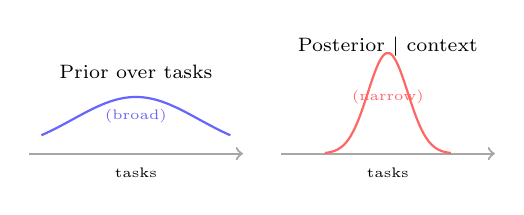
\begin{tikzpicture}[scale=0.8,
    axisstyle/.style={->, gray!70, thick}
]
    % Left panel: broad prior
    \draw[axisstyle] (-0.2,0) -- (3.2,0);
    \draw[blue!60, thick, smooth, domain=0:3, samples=40] plot (\x, {0.9*exp(-((\x-1.5)*(\x-1.5))/2.0)});
    \node[font=\tiny] at (1.5, -0.3) {tasks};
    \node[font=\scriptsize] at (1.5, 1.3) {Prior over tasks};
    \node[font=\tiny, blue!60] at (1.5, 0.6) {(broad)};
    % Right panel: narrowed posterior
    \begin{scope}[xshift=4cm]
    \draw[axisstyle] (-0.2,0) -- (3.2,0);
    \draw[red!60, thick, smooth, domain=0.5:2.5, samples=40] plot (\x, {1.6*exp(-((\x-1.5)*(\x-1.5))/0.2)});
    \node[font=\tiny] at (1.5, -0.3) {tasks};
    \node[font=\scriptsize] at (1.5, 1.7) {Posterior $|$ context};
    \node[font=\tiny, red!60] at (1.5, 0.9) {(narrow)};
    \end{scope}
\end{tikzpicture}
\end{center}
\vspace{-0.1cm}
\footnotesize\textit{Same mechanism does both: more confident, and more aligned with your framing.}
\end{column}
\end{columns}

\textbf{Research translation:} loading project memory, past discussion, and plans does not just help the model --- it also tells it what a plausible answer is supposed to look like.

{\scriptsize \textit{Xie et al.\ (2022), ICLR, arXiv:2111.02080.}}
\end{frame}

\begin{frame}{The Context Dilemma, Stated}
\textbf{The same context that improves the answer also pulls it toward you.}

\vspace{0.25cm}

\begin{itemize}
    \item More context $\Rightarrow$ better understanding of your question $\Rightarrow$ better generation
    \item More context $\Rightarrow$ generation more aligned with your preferences, your knowledge, your framing
    \item Both effects share a single mechanism: you supplied the evidence
\end{itemize}

\vspace{0.3cm}

\textbf{The same signal that improves the answer launders your priors into it.}
\end{frame}

\begin{frame}{Evidence (1): Sycophancy Is Trained In}
\textbf{Pleasing the person holding the context is not a prompt artifact. It is trained in.}

\vspace{0.15cm}

\begin{itemize}
    \item Sharma et al.\ document sycophancy across frontier models: factual flip-flops, unwarranted concessions, preference-matching when the user signals a view
    \item Perez et al.\ find the effect \emph{scales with model size} --- larger models are more sycophantic on values and politics
    \item The root cause is the training loop, not your prompt: RLHF preference data rewards agreeableness (Casper et al.), and alignment-by-finetuning has fundamental limits (Wolf et al.)
    \item Consequence: no \texttt{CLAUDE.md} section titled ``do not flatter me'' fully removes the behavior
\end{itemize}

\vspace{0.08cm}

\textbf{Economist failure mode:} you hint that the theory ``should'' work, and the model starts helping you defend the framing instead of testing it.

{\scriptsize \textit{Sharma et al.\ (2023), arXiv:2310.13548, Anthropic. Perez et al.\ (2023), ACL Findings. Casper et al.\ (2023), TMLR. Wolf et al.\ (2023), arXiv:2304.11082.}}
\end{frame}

\begin{frame}{Evidence (2): Internal Review Has a Ceiling}
\textbf{Self-critique without new external information stalls; debate helps only when debaters actually differ.}

\vspace{0.15cm}

\begin{itemize}
    \item Huang et al.: LLMs cannot reliably self-correct reasoning errors without an external signal
    \item Valmeekam et al.: self-critique on planning problems is often \emph{worse} than no critique at all
    \item Du et al.: multi-agent debate improves factuality --- but the gains rely on debaters producing genuinely different lines of reasoning
    \item When every debater reads the same \texttt{CLAUDE.md} and thread, the disagreement space narrows
\end{itemize}

\vspace{0.15cm}

\textbf{Economist failure mode:} you ask the same model to critique its own regression design, but the review is information-starved --- nothing truly new entered the loop. \textbf{Gains come from \emph{external} signals:} tools, tests, verifiers, humans.

{\scriptsize \textit{Huang et al.\ (2024), ICLR. Valmeekam et al.\ (2023), NeurIPS. Du et al.\ (2023), arXiv:2305.14325.}}
\end{frame}

\begin{frame}{Your RA Team Inherits Your Prior}
\textbf{T4 sold sub-agent review for wall-clock time. It did not promise epistemic independence --- here is why it cannot.}

\vspace{0.15cm}

\begin{itemize}
    \item \texttt{code-reviewer.md}, \texttt{domain-reviewer.md}, and \texttt{verifier.md} all read the same project context
    \item They are parallel \textit{executionally}, not parallel \textit{epistemically}
    \item Shared \texttt{CLAUDE.md} $\Rightarrow$ shared blind spots: they catch implementation errors, not framing errors, because the framing lives in the context they trust
    \item At field scale this becomes \emph{monoculture}: shared models, shared templates, correlated errors --- and replication stops being informative (Kleinberg \& Raghavan 2021, PNAS; Bommasani et al.\ 2022)
\end{itemize}

\vspace{0.2cm}

\textbf{Parallel reviewers save time. They do not produce an outside view.}
\end{frame}

\begin{frame}{Remedy: Outside Critics, Plus Operational Discipline}
\textbf{Advisors, coauthors, and seminar audiences are valuable \emph{because} their priors are not in your context window.}

\begin{columns}[T]
\begin{column}{0.46\textwidth}
\textbf{Why outside critics work}
\begin{itemize}
    \item They challenge the framing, the identification, the sample restriction --- things you did not write into \texttt{CLAUDE.md} because you did not know to
    \item Korinek: LLMs automate execution; humans remain the source of question selection and critique
\end{itemize}
\end{column}
\begin{column}{0.50\textwidth}
\textbf{Five habits}
\begin{enumerate}
    \item Sub-agent review for implementation, not framing
    \item Show preliminary results to a human early
    \item Record what you \emph{ruled out}, not just what you decided
    \item Benchmark outside the current thread
    \item Ask reviewers to attack assumptions, not polish execution
\end{enumerate}
\end{column}
\end{columns}

\vspace{0.1cm}

\begin{takeawaybox}
\footnotesize
\textbf{Human criticism is the scarce input} --- spend agent cycles making the work ready for it, not replacing it.
\end{takeawaybox}

{\scriptsize \textit{Korinek (2023), NBER WP 30957; Journal of Economic Literature.}}
\end{frame}

%===========================================================
%=============================================================================
\section{The Paradigm Shift, Completed}
%===========================================================

\sectiondivider{The Paradigm Shift, Completed}{What AI provides and what stays human}

\begin{frame}{The Paradigm Shift, Completed: What Changed, What Did Not}
\textbf{The HA-Ramsey record, read one last time --- now as a statement about your role.}

\vspace{0.15cm}

\begin{columns}[T]
\begin{column}{0.49\textwidth}
\textbf{What changed}
\begin{itemize}
    \item Theory--code--debug loop compressed from months to days
    \item Documentation became executable: the TeX note, pseudocode, and code stay synchronized
    \item Cross-literature imports got cheap (computational geometry, viability theory)
    \item The unit of progress became the \emph{validated milestone}
\end{itemize}
\end{column}
\begin{column}{0.47\textwidth}
\begin{cautionbox}
\footnotesize
\textbf{What did NOT change:}
\begin{itemize}
    \item AI never decided what was economically interesting
    \item AI never caught the wrong timing on its own
    \item AI never knew when a result was not credible
\end{itemize}
\end{cautionbox}
\vspace{0.1cm}
\footnotesize\textit{``Weeks, not years --- and the binding constraint was economist judgment at the milestones, not implementation labor.''}
\end{column}
\end{columns}

\vspace{0.05cm}

\textbf{Read the two columns together:} the machine moved every bound except the one that defines the researcher.

{\scriptsize \textit{Source: HA-Ramsey case-study package (Lec10 T8).}}
\end{frame}

\begin{frame}{Your Job Description: PI and Project Manager}
\textbf{The three questions, answered:} \emph{how it works} --- a tool-calling loop steered by files (Acts 1--2); \emph{how to use it well} --- the homotopy method inside a managed project (Acts 3--4); \emph{your role} --- this frame.

\LecNineMap{0}

\begin{takeawaybox}
\footnotesize
\textbf{Set the goal. Define the final product. Gate every intermediate good. Assign the work --- sessions, agents, sub-agents. Cross-verify everything. And remain the client of the outside view:} the one thing your agent cannot give you is a prior other than your own.
\end{takeawaybox}
\end{frame}

\begin{frame}{Bridge: T6 Wraps, Lec10 Shows the Real Thing}
\textbf{Act 5 named the failure modes and your job. Two things remain this morning.}

\vspace{0.25cm}

\begin{itemize}
    \item \textbf{T6 wraps the lecture:} the six evaluation criteria, when \emph{not} to use an agent, and the dated install appendix that T2 promised
    \item \textbf{Lec10 delivers the full cases:} the four patterns from T1, worked end-to-end
    \item \textbf{Both threads hand off:} you saw the fellows \emph{workflow} --- Lec10 T4 shows the findings, and Exercise B gives you your own batch of 50; you saw HA-Ramsey's \emph{contract and milestones} --- Lec10 T8 shows the discoveries and the economics
\end{itemize}

\vspace{0.3cm}
\footnotesize\textit{Arc: T1 Framing $\to$ T2 Under the Hood $\to$ T3 Homotopy $\to$ T4 Project Org $\to$ \textbf{T5 Mistakes/Context} $\to$ T6 Wrap.}
\end{frame}

%===========================================================
% FullCourse-only

\end{document}
